\chapter{WAVELENGTH-MODULATION SPECTROSCOPY TECHNIQUES}

Wavelength modulation spectroscopy (WMS) is a well-known and widely used LAS technique that offers several noise rejection benefits, making it well-suited for hostile environments and applications with small absorbance. In WMS, the laser intensity and wavelength are modulated sinusoidally at frequency $f_m$, using TDLs and other semiconductor lasers (e.g., quantum-cascade lasers). This is achieved via injection-current modulation. The wavelength modulation shifts absorption information to harmonics of the modulation frequency. Because the modulation frequency is usually very high (near $MHz$), absorption information can be isolated from low-frequency noise (e.g., from electronics or environmental factors). Moreover, all harmonics signals are linearly proportional to the DC laser intensity. As a result, the second-harmonic signal (2$f_m$), which is dominated by absorption, can be normalized by the first-harmonic signal (1$f_m$), which is dominated by laser-intensity modulation, to provide WMS-$2f/1f$ signals that are independent of the DC light intensity. This technique has significant advantages in harsh environment, since the WMS-$2f/1f$ signal is insensitive to noise from beam steering, window fouling, etc.  In this chapter, two WMS techniques known as 	``fixed-WMS'' and ``scanned-WMS'' are discussed.

%WMS can achieve gas measurements with relatively low absorbance down to $10^{-5}$.


 \section{Fixed-WMS}
In fixed-WMS, the laser wavelength is sinusoidally modulated while it is centered on an absorption transition linecenter. This leads to a WMS-$2f/1f$ signal that is constant in time (for constant gas conditions), much like a fixed-wavelength direct-absorption measurement. To convert measured WMS-$2f/1f$ signals to measurements of gas properties, a calibration-free WMS model is required to predict how WMS signals vary with gas conditions ($T$,$P$,$\chi$). In this work, fixed-WMS signals were simulated using the calibration-free WMS model developed by Rieker et al. \cite{rieker2009calibration}. 

In this model, the laser wavelength modulation is modeled according to:
\begin{equation}
\nu(t)=\overline{\nu}+a\,cos(wt) \quad [cm^{-1}]
\end{equation}
\begin{equation}
w=2\pi f_m
\end{equation}

\noindent $\overline{\nu}$ is the center frequency, and $a$ is the modulation depth (i.e., amplitude). The laser's incident laser intensity is modeled to $2^{nd}$ order, according to: 
\begin{equation}
I_0(t)=\overline{I_0}(1+\underbrace{i_0\,cos(wt+\psi_1)}_{1f\,term}+\underbrace{i_2\,cos(wt+\psi_2)}_{2f\,term})
\end{equation}

\noindent Here, $\overline{I_0}$ is the average incident intensity, $i_0$ and $i_2$ are linear and nonlinear amplitudes (normalized by $\overline{I_0}$). $\psi_1$ and $\psi_2$ are the phase shifts between intensity modulation and frequency modulation for both intensity modulation terms. The laser intensity modulation is modeled to $2_{nd}$-order to account for the laser's non-linear response to current modulation, which leads to a small but non-zero WMS-$2f$ background signal. Using this approach, the laser background signal is accounted for in the WMS model. All of the aforementioned laser modulation parameters are measured in laboratory experiments and input into the model as discussed by Rieker et al. \cite{rieker2009calibration}.

A transmission coefficient $\tau$ is defined to quantify the fraction of laser light that is absorbed when traveling through the test gas. $\tau$ depends on gas properties and instantaneous laser frequency with the following expression:
\begin{equation}
\tau(\nu(t))=exp\{-\alpha[\nu(t)]\}=exp[-\sum_{j}S_j(T)P\chi L\phi_j(\nu(t))]
\end{equation}

The transmission coefficient $\tau$ can also be expressed as a Fourier series:
\begin{equation}
\tau(\nu(t))=\frac{I_t(\nu(t))}{I_0(\nu(t))}=\sum_{k=0}^{\infty}H_k(\overline{\nu},a)cos(kwt)=H_0+\sum_{k=1}^{\infty}H_k(\overline{\nu},a)cos(kwt)
\end{equation}

\noindent Here Fourier coefficients $H_0$ and $H_k$ are given by:
\begin{equation}
H_0(T,P,\overline{\nu},a)=\frac{1}{2\pi}\int_{-\pi}^{\pi}\exp\{-\sum_j\,S_j(T) \cdot \phi_j(T,P,\chi,\overline{\nu}+a\,cos\theta) \cdot P \cdot \chi \cdot L\}\,d\theta
\end{equation}
\begin{equation}
H_k(T,P,\overline{\nu},a)=\frac{1}{\pi}\int_{-\pi}^{\pi}exp\{-\sum_j\,S_j(T) \cdot \phi_j(T,P,\chi,\overline{\nu}+a\,cos\theta) \cdot P \cdot \chi \cdot L\}cos k\theta d\theta
\end{equation}

Hence the transmitted laser intensity can be modeled using Eq. (3.8). It is noted that $H_0$ term is equivalent to transmission coefficient at center frequency $\overline{\nu}$. $H_k$ terms are related to the $k$th derivative of transmission coefficient function.  
\begin{equation}
I_t(t)=I_0(t)\tau[\nu(t)]=\overline{I_0}(1+i_0\,cos(wt+\psi_1)+i_1\,cos(wt+\psi_2))(H_0+\sum_{k=1}^{\infty}H_k(\overline{\nu},a)cos(kwt))
\end{equation}

In experiments, a lock-in filter or amplifier is used to extract the X and Y components of the WMS-$1f$ and -$2f$ signals from the measured detector signal. This is illustrated by Fig. 3.1. In the calibration-free WMS model, the X and Y components of the $1f$ and $2f$ signal can be calculated from the Fourier coefficients using Eq. (3.9) through Eq. (3.12).
%$nf_m$ ($nth$ harmonics) signals from the detector. After receiving transmitted signals from detector, the signals carry out the fast Fourier transform and then are multiplied by a sinusoidal function at frequency $nf_m$. Corresponding harmonics signals are isolated and simulated as $S=X+iY$, where X component is obtained by multiplication of $cos2\pi nf_mt$ and Y component by multiplication of $sin2\pi nf_mt$ (Fig 3.1).  Simplified forms of X and Y components for $1f$ and $2f$ signals are demonstrated in Eqn 3.9 - Eqn 3.12.

\begin{equation}
X_1f=\frac{G\overline{I_0}}{2}[H_1+i_0(H_0+\frac{H_2}{2})cos\psi_1+\frac{i_2}{2}(H_1+H_3)cos\psi_2]
\end{equation}
\begin{equation}
Y_1f=-\frac{G\overline{I_0}}{2}[i_0(H_0-\frac{H_2}{2})sin\psi_1+\frac{i_2}{2}(H_1-H_3)sin\psi_2]
\end{equation}
\begin{equation}
X_2f=\frac{G\overline{I_0}}{2}[H_2+\frac{i_0}{2}(H_1+H_3)cos\psi_1+i_2(H_0+\frac{H_4}{2})cos\psi_2]
\end{equation}
\begin{equation}
Y_2f=-\frac{G\overline{I_0}}{2}[\frac{i_0}{2}(H_1-H_3)sin\psi_1+i_2(H_0-\frac{H_4}{2})sin\psi_2]
\end{equation}

\noindent Here, $G$ denotes the electro-optical gain of the detection system. This term will be canceled out by performing 1-$f$ normalization. The magnitude of the WMS harmonic signal ($S_{nf}$) is given by Eq. (3.13):
\begin{equation}
S_{nf}=\sqrt[]{X_{nf}^2+Y_{nf}^2}
\end{equation}

 \begin{figure}[h]
    \centering
        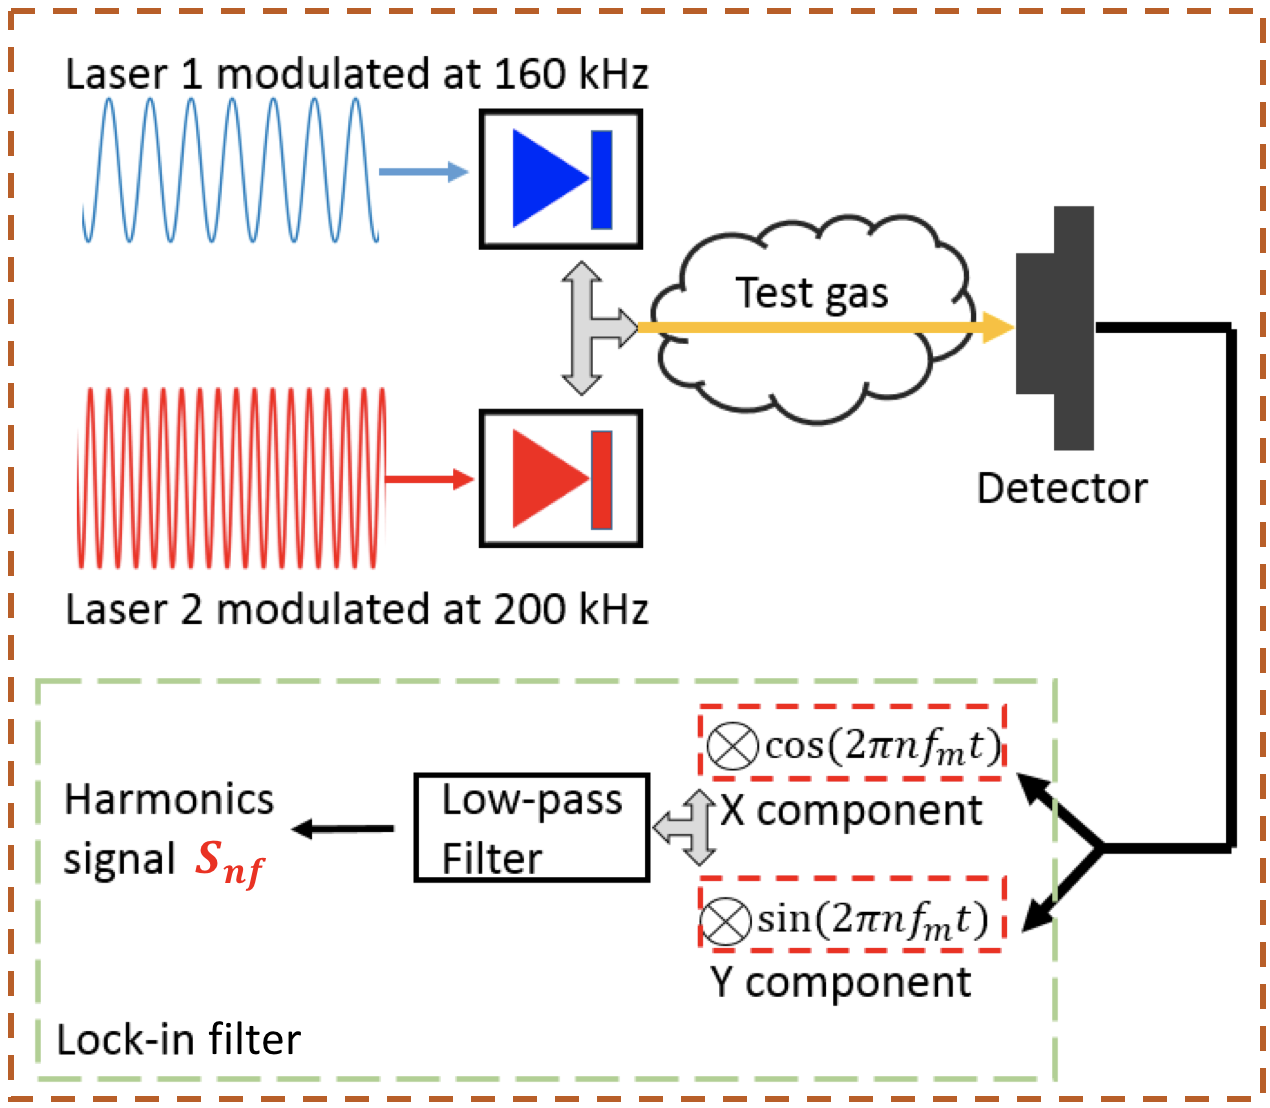
\includegraphics[width=0.85\textwidth]{fig/ch3_fig1_v3.png}
        \caption{Schematic illustrating how WMS harmonic signals are extracted from the detector signal during post-processing.}
    \label{fig:ch3_1}
\end{figure}

As mentioned previously, the WMS-$2f/1f$ signal is immune to variations in DC light intensity (e.g., from beam steering, window fouling, scattering, etc). The absolute value of the WMS-$2f/1f$ signal can be calculated using the calibration-free model according to:
\begin{equation}
S_{2f/1f}=\frac{S_{2f}}{S_{1f}}=\frac{\sqrt[]{X_{2f}^2+Y_{2f}^2}}{\sqrt[]{X_{1f}^2+Y_{1f}^2}}
\end{equation}

It should be noted that $1f$ and $2f$ signals are not zero when the absorption is zero due to the background signals resulting from linear and nonlinear intensity modulation. However, $i_2$ is typically small ($\approx \, \frac{i}{100}i_0$) leading to a near-zero WMS-$2f$ background. When the absorption is zero, the $H_0$ term is equal to 1 and 0 for $H_k$ ($k\neq 0$), which produces the following X and Y components:

\begin{equation}
X_{1f}^0=\frac{\overline{I_0}}{2}i_0cos\psi_1
\end{equation}
\begin{equation}
Y_{1f}^0=-\frac{\overline{I_0}}{2}i_0sin\psi_1
\end{equation}
\begin{equation}
X_{2f}^0=\frac{\overline{I_0}}{2}i_2cos\psi_2
\end{equation}
\begin{equation}
Y_{2f}^0=-\frac{\overline{I_0}}{2}i_2cos\psi_2
\end{equation}

 \begin{figure}[h]
    \centering
        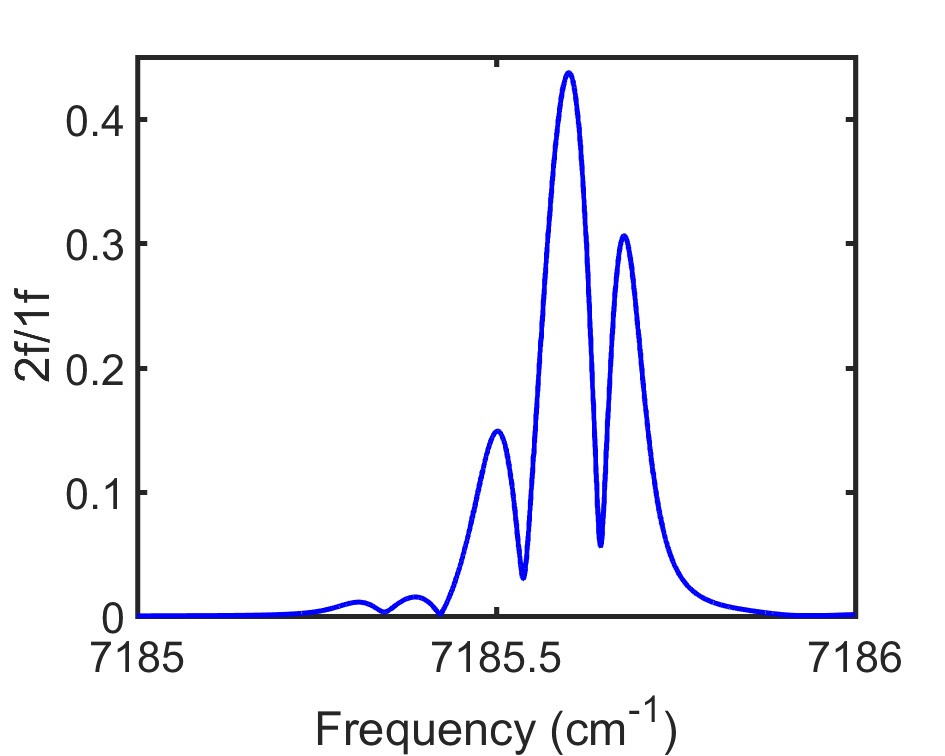
\includegraphics[width=0.7\textwidth]{fig/ch3_fig2.png}
        \caption{Simulated WMS-$2f/1f$ signal for a $H_2O$ absorption transition near 1392 nm. The calibration-free model developed by Rieker et al \cite{rieker2009calibration} was used.}
    \label{fig:ch3_1}
\end{figure}

Thus, the background signals are nonzero under absorption-free conditions. In practical applications, these background signals need to be subtracted using the following expression:
\begin{equation}
S_{2f/1f}=\sqrt[]{\left[\left(\frac{X_{2f}}{S_1f}\right)_{raw}-\left(\frac{X_{2f}}{S_1f}\right)_{bg}\right]^2+\left[\left(\frac{Y_{2f}}{S_1f}\right)_{raw}-\left(\frac{Y_{2f}}{S_1f}\right)_{bg}\right]^2}
\end{equation}

\noindent where the subscripts ``raw'' and ``bg'' refer to signals with absorption and laser background and only laser background, respectively.

\section{Scanned-WMS-$2f/1f$}
In scanned-WMS, the laser wavelength is simultaneously modulated and scanned sinusoidally over the absorption feature to obtain WMS spectra, which can improve measurement accuracy. This is directly analogous to direct-absorption techniques. Scanned-WMS has been applied extensively to provide gas property (e.g. $T$, $P$, $\chi$) measurements in harsh environments \cite{Goldenstein2017,Ma2013,Caswell2013,Stritzke2015,Witzel2013,Whitney2011,Makowiecki2017,Rieker2009b,Li2011}. Among scanned-WMS, ``peak-picking scanned-WMS'' and ``full-spectrum scanned-WMS'' have been used to characterize several combustion applications \cite{WOLFRUM19981,HANSON20111,Goldenstein2017,hanson2016spectroscopy,Schulz2007}. In peak-picking scanned-WMS, the laser wavelength is scanned with a small amplitude to obtain only the peak value of the WMS-$2f/1f$ signal near the transition linecenter. This technique provides a known wavelength reference and therefore improves measurement accuracy compared to fixed-WMS \cite{goldenstein20151}. More recently, Goldenstein et al. \cite{Goldenstein2014} developed a calibration-free scanned-WMS-$2f/1f$ spectral-fitting technique which can be applied to full-spectrum scanned-WMS. This spectral-fitting technique does not need \textit{a priori} knowledge of line-broadening information, thus providing advantages in many practical applications where gas conditions and, thus, collisional broadening, are unknown. This technique was used by the single-ended LAS sensor presented in Chapter 4. 

 \begin{figure}[h]
    \centering
        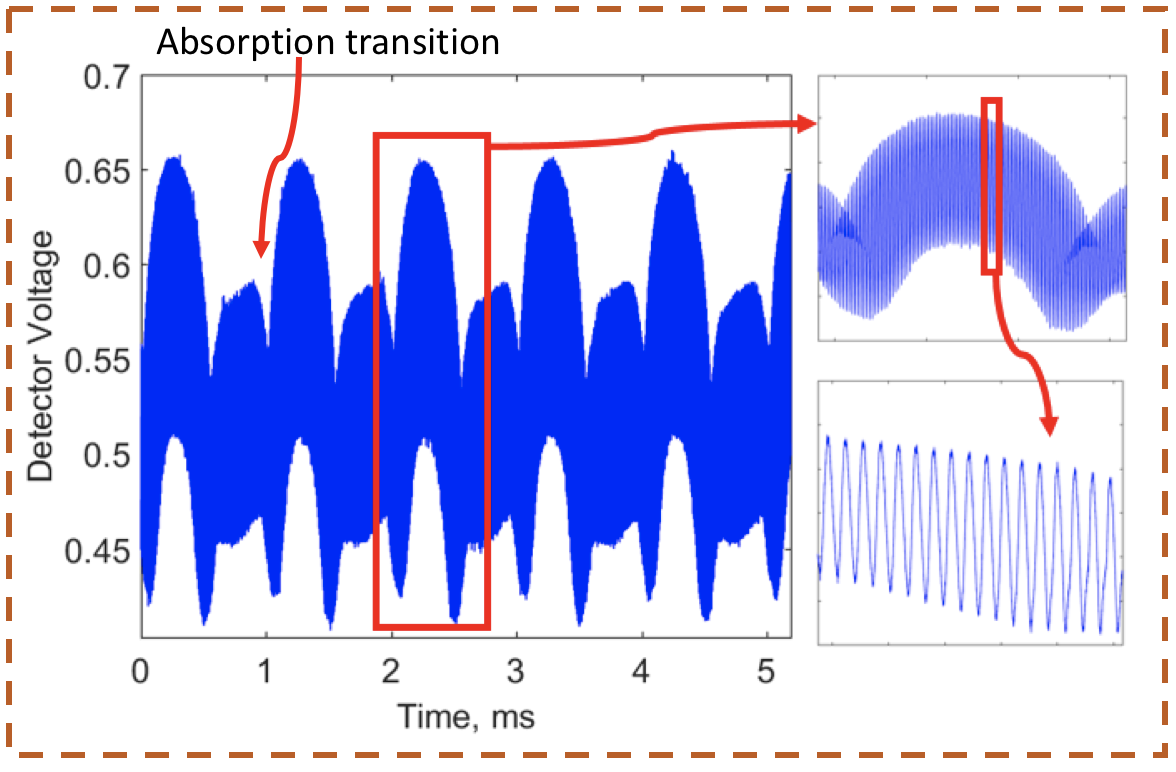
\includegraphics[trim = 0mm 0mm 0mm 0mm, clip=true, width=0.8\textwidth]{fig/ch3_fig3_v2.png}
        \caption{An example of measured detector signal in a scanned-WMS experiment.The laser current is scanned at a frequency of 1 $kHz$ and modulated at a frequency of 160 $kHz$. Subpanels show scan and modulation envelopes in detail.}
    \label{fig:ch4_1}
\end{figure}

Compared to fixed-WMS, in scanned-WMS the incident laser intensity is simulated with an additional sinusoidal signal due to the scan waveform applied to the laser's injection current. In general the scan frequency is $\approx100x$ smaller than the modulation frequency. The incident laser intensity is modeled as:
\begin{equation}
I_0(t)=I_{0,S}(t)+I_{0,M}(t)
\end{equation}

\noindent Here $I_{0,S}$ and $I_{0,M}$ denotes the laser intensity's response to current scanning and modulation respectively. Fig. 3.3 shows an example of the detector signal in a scanned-WMS experiment. The figure shows how the scan and modulation superimpose on each other and how the laser intensity decreases as the laser wavelength is scanned across an absorption transition. The time varying laser frequency can be modeled in a similar manner according to:


\begin{equation}
\nu(t)=\overline{\nu}+\nu_S(t)+\nu_M(t)
\end{equation}
\begin{equation}
\nu_S(t)=a_{1,S}sin(w_St+\psi_{1,S})+a_{2,S}sin(2w_St+\psi_{2,S})
\end{equation}
\begin{equation}
\nu_M(t)=a_{1,M}sin(w_Mt+\psi_{1,M})+a_{2,M}sin(2w_Mt+\psi_{2,M})
\end{equation}

%\vspace{10mm}

\noindent where $\overline{\nu}$ is the line center frequency of the laser. Similar to Eq. (3.3), $a_1$ and $a_2$ represent modulation depths for $1^{st}$ and $2^{nd}$ order, however, it should be noted that $a_{2,S}$ is typically 100$x$ smaller than $a_{1,S}$ and can be ignored in most cases. $\psi_1$ and $\psi_2$ are the phase shift between wavelength and intensity modulation for $1^{st}$ and $2^{nd}$ order terms respectively. After simulating $I_0(t)$ and $\nu(t)$, the time-varying transmitted intensity $I_t(t)$ can be determined using the Beer Lambert relation.
\begin{equation}
I_t(t)=I_0(t)exp[-\phi(\nu(t),T,P,\chi)A]
\end{equation}
Here $A$ represents the integrated absorbance given by:
\begin{equation}
A=\int_{-\infty}^{\infty}\alpha(\nu) d\nu=S(T)P\chi_iL
\end{equation}

 \begin{figure}[h]
    \centering
        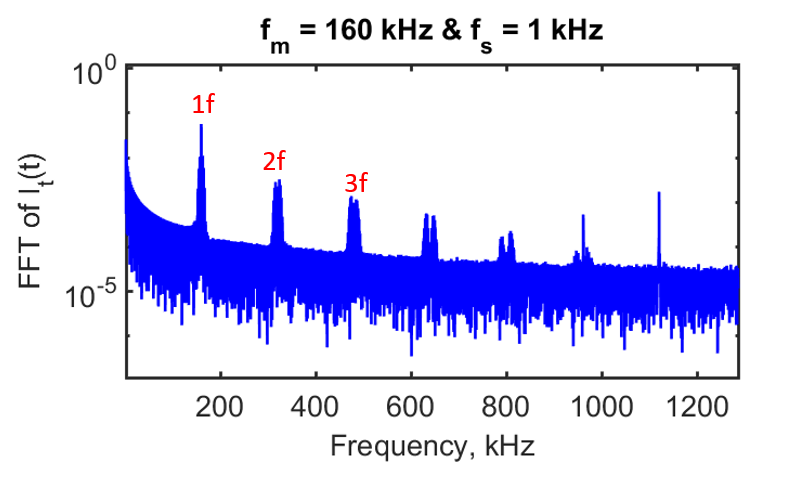
\includegraphics[trim = 0mm 0mm 0mm 0mm, clip=true, width=0.9\textwidth]{fig/ch3_fig5.png}
        \caption{FFT of a measured detector signal for a scanned-WMS-$2f/1f$ experiment. The laser is sinusoidally modulated at the frequency of 160 kHz and scanned at the frequency of 1 kHz. The first three harmonic signals are marked in the picture where $1f$ = 160 kHz, $2f$ = 320 kHz and $3f$ = 480 kHz. The scan waveform introduces sidebands centered around each harmonic.}
    \label{fig:ch3_4}
\end{figure}

After calculating $I_t$, the simulated scanned-WMS-$2f/1f$ signal can be extracted from $I_t$ using a digital lock-in filter. Fig. 3.4 shows a the frequency spectrum of a measured detector signals. The X and Y components of the first two harmonic signals can be isolated and extracted with digital lock-in filters. The magnitude of the WMS-$2f/1f$ signal can then be calculated using Eq. (3.26):

\begin{equation}
S_{2f/1f}=\frac{\sqrt[]{X_{2f}^2+Y_{2f}^2}}{\sqrt[]{X_{1f}^2+Y_{1f}^2}}=f(laser\,parameters,A,\Delta\nu_C,\Delta\nu_D,\nu_0)
\end{equation}

\vspace{3mm}
\noindent which shows that $S_{2f/1f}$ is a function if laser parameters and spectroscopy quantities.

 \begin{figure}[h]
    \centering
        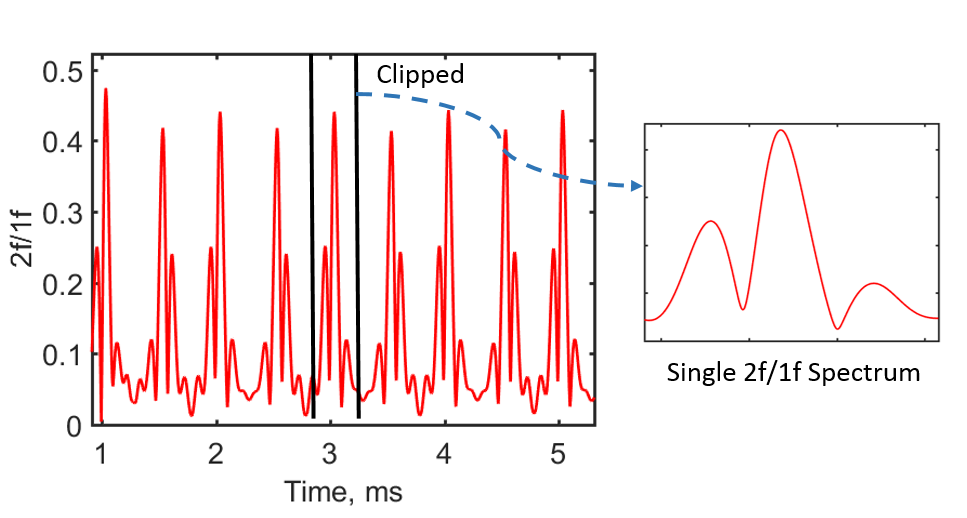
\includegraphics[trim = 0mm 0mm 0mm 0mm, clip=true, width=0.8\textwidth]{fig/ch3_fig6.png}
        \caption{Left: WMS-$2f/1f$ signal time history for a scanned-WMS experiment. The laser is modulated at 160 kHz and scanned at 1000 Hz. It is noted that WMS-$2f/1f$ signals are slightly different for up-scan and down-scan due to the phase-shift between the laser intensity and wavelength. Right: Clipped single spectrum. Spectral fitting is applied to each single spectrum to infer gas properties.}
    \label{fig:ch3_5}
\end{figure}

 \begin{figure}[h]
    \centering
        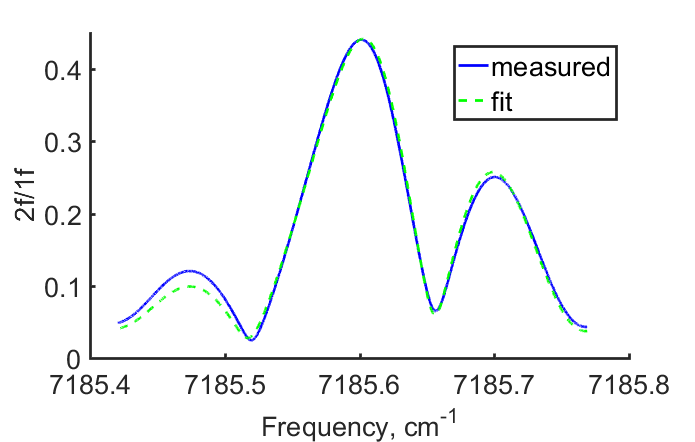
\includegraphics[width=0.7\textwidth]{fig/ch3_fig7.png}
        \caption{An example of a single scanned-WMS-$2f/1f$ spectrum and its best fit. The fitting has a peak-normalized residual less than 4$\%$.}
    \label{fig:ch3_6}
\end{figure}

\vspace{30mm}


Fig. 3.5 illustrates an example of a measured scanned-WMS-$2f/1f$ signal time history. A single spectrum (for an up-scan or down-scan) can then be extracted from the time history and fed to a WMS-$2f/1f$ spectral fitting routine. Here, the spectral-fitting technique developed by Goldenstein et al. \cite{Goldenstein2017} was used in a non-linear least-squares fitting routine to determine the best-fit spectrum and spectroscopic quantities. In this technique, the aforementioned scanned-WMS simulation technique is incorporated into a non-linear least-squares fitting routine. The laser modulation parameters (determined from controlled laboratory experiments), and the Doppler width ($\Delta\nu_D$) are fixed, and $\nu_0$, $A$, and $\Delta\nu_C$ are free-parameters that manipulate the simulated WMS-$2f/1f$ spectrum. Fig. 3.6 shows an example of a measured WMS-$2f/1f$ spectrum and its best fit for an $H_2O$ absorption transition near 7185.6 $cm^{-1}$. The value of $A$ corresponding to the best-fit spectrum is used to determine the absorbing species mole fraction and/or gas temperature analogous to scanned-wavelength direct absorption.


%\section{Characterization of Diode Lasers}

